\documentclass{sig-alternate}
\usepackage[USenglish]{babel}
\usepackage[backend=bibtex,style=numeric-comp]{biblatex}
\usepackage{tikz}
\usetikzlibrary{positioning}

\newcommand{\code}[1]{\texttt{#1}}

\author{
\alignauthor{}
Dan Stelljes\\
  \affaddr{Division of Science and Mathematics}\\
  \affaddr{University of Minnesota, Morris}\\
  \affaddr{Morris, Minnesota, USA 56267}\\
  \email{stell124@morris.umn.edu}
}
\conferenceinfo{UMM CSci Senior Seminar Conference, December 2016}{Morris, MN}
\title{Composable Concurrency Models}

\bibliography{references}

\AtEveryBibitem{\clearfield{doi}}
\AtEveryBibitem{\clearfield{note}}

\begin{document}

\maketitle

\begin{abstract}

The need to manage concurrent operations in applications has led to the development of a variety of concurrency models. Modern programming languages generally provide several concurrency models to serve different requirements, and programmers benefit from being able to use them in tandem. We discuss challenges surrounding concurrent programming and examine situations in which conflicts between models can occur. Additionally, we describe attempts to identify features of common concurrency models and develop lower-level abstractions capable of supporting a variety of models.

\end{abstract}

\section{Introduction}

Most interactive computer programs depend on concurrency, the ability to perform different tasks at the same time. A web browser, for instance, might at any point be rendering documents in multiple tabs, transferring files, and handling user interaction. On a lower level, the operating system might be running several other applications, juggling background processes, and responding to events. If every long-running process blocked other processes from proceeding, the system would be effectively unusable.

Processes themselves are often composed of multiple concurrent threads of execution that each work on a distinct task. A processor can only execute one thread at a time, so multitasking is accomplished by rapidly switching between threads~\cite{Liu1973}. Although concurrent threads may appear to be executed simultaneously, truly parallel execution can only take place across multiple processors.

Concurrency models enable programmers to reason about concurrent tasks instead of low-level thread management. The web browser is a good example of how different models might be chosen to represent specific types of tasks: The user interface layer might rely on an event loop, the rendering process might operate in shared memory, and suggestions from browsing history or a search engine might require parallel collection operations to achieve acceptable performance~\cite{Marr2012}.

Given that an application is likely to make use of more than one concurrency model, programmers would prefer that different types of models could safely interact. However, different models do not necessarily work well together, nor are they designed to. Recent work has attempted to identify common ``building blocks'' that could be used to compose a variety of models, possibly eliminating subtle problems when different models interact and allowing models to be represented at lower levels without resorting to rough approximations~\cite{Marr2012, Swalens2014, Ziv2015}.

\section{Background}

In a concurrent program, the history of operations may not be the same for every execution. An entirely sequential program could be proved to be correct by showing that its history (that is, the sequence in which its operations are performed) always yields a correct result. For a concurrent program to be proved correct, though, it must be clear that all possible histories always yield a correct result. Furthermore, concurrent programming frequently involves the use of shared resources that require coordinated access and manipulation.

Consistency models, restrictions on possible execution histories, can guarantee that a program will produce a correct result~\cite{Ziv2015}. If an execution of a program follows an allowed history, that execution is said to be consistent; if not, it is said to be inconsistent. If every possible execution of the program is guaranteed to follow a history allowed by a consistency model, that program conforms to that consistency model~\cite{Kingsbury2014}.

\begin{figure}[ht]
  \centering
  \resizebox{0.95\linewidth}{!}{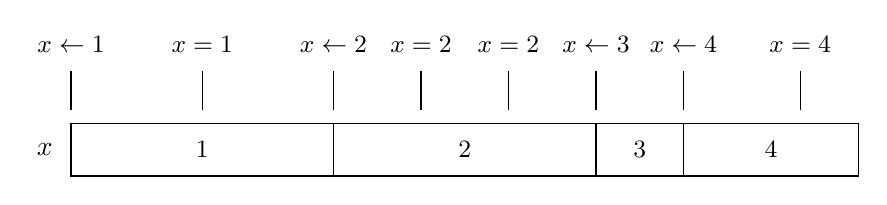
\begin{tikzpicture}
  \node at (-5.333,0) { $x$ };

  \draw (-5,-0.333) rectangle (-1.667,0.333) node [midway] { \small $1$ };
  \draw (-1.667,-0.333) rectangle (1.667,0.333) node [midway] { \small $2$ };
  \draw (1.667,-0.333) rectangle (2.778,0.333) node [midway] { \small $3$ };
  \draw (2.778,-0.333) rectangle (5,0.333) node [midway] { \small $4$ };

  \draw (-5,0.5) -- (-5,1) node [above=3pt] { \small $x \leftarrow 1$ };
  \draw (-3.333,0.5) -- (-3.333,1) node [above=3pt] { \small $x = 1$ };

  \draw (-1.667,0.5) -- (-1.667,1) node [above=3pt] { \small $x \leftarrow 2$ };
  \draw (-0.555,0.5) -- (-0.555,1) node [above=3pt] { \small $x = 2$ };
  \draw (0.555,0.5) -- (0.555,1) node [above=3pt] { \small $x = 2$ };

  \draw (1.667,0.5) -- (1.667,1) node [above=3pt] { \small $x \leftarrow 3$ };

  \draw (2.778,0.5) -- (2.778,1) node [above=3pt] { \small $x \leftarrow 4$ };
  \draw (4.26,0.5) -- (4.26,1) node [above=3pt] { \small $x = 4$ };
\end{tikzpicture}
}
  \caption{A single thread reads from and writes to a variable.}
\label{figure:single}
\end{figure}

Figure~\ref{figure:single} illustrates a simple program in which a single thread $A$ reads ($=$) and writes ($\leftarrow$) values on a variable $x$, denoted by a segmented bar containing the value of $x$ over time. The program satisfies an intuitive model of how variables should behave---each time $x$ is read, the value returned is equal to the value most recently written and the consistency model holds. If, however, a read on $x$ failed to return the most recently written value, the consistency model would be violated.

\begin{figure}[ht]
  \centering
  \resizebox{0.85\linewidth}{!}{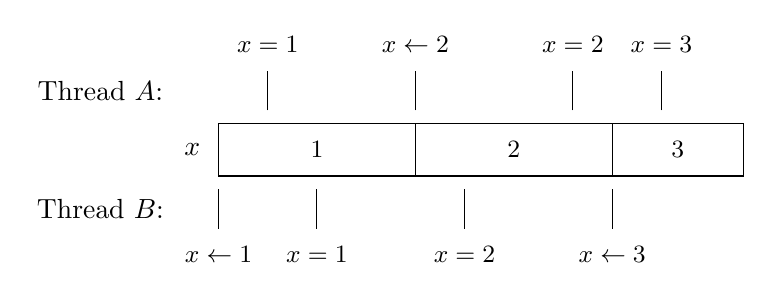
\begin{tikzpicture}
  \node at (-6.5,0.75) { Thread $A$: };
  \node at (-6.5,-0.75) { Thread $B$: };
  \node at (-5.333,0) { $x$ };

  \draw (-5,-0.333) rectangle (-2.5,0.333) node [midway] { \small $1$ };
  \draw (-2.5,-0.333) rectangle (0,0.333) node [midway] { \small $2$ };
  \draw (0,-0.333) rectangle (1.667,0.333) node [midway] { \small $3$ };

  \draw (-5,-0.5) -- (-5,-1) node [below=3pt] { \small $x \leftarrow 1$ };
  \draw (-4.375,0.5) -- (-4.375,1) node [above=3pt] { \small $x = 1$ };
  \draw (-3.75,-0.5) -- (-3.75,-1) node [below=3pt] { \small $x = 1$ };

  \draw (-2.5,0.5) -- (-2.5,1) node [above=3pt] { \small $x \leftarrow 2$ };
  \draw (-1.875,-0.5) -- (-1.875,-1) node [below=3pt] { \small $x = 2$ };
  \draw (-0.5,0.5) -- (-0.5,1) node [above=3pt] { \small $x = 2$ };

  \draw (0,-0.5) -- (0,-1) node [below=3pt] { \small $x \leftarrow 3$ };
  \draw (0.625,0.5) -- (0.625,1) node [above=3pt] { \small $x = 3$ };
\end{tikzpicture}
}
  \caption{Two threads concurrently read from and write to a variable.}
\label{figure:multiple}
\end{figure}

In Figure~\ref{figure:multiple}, two threads $A$ and $B$ concurrently read and write on $x$. Because the operations of the threads are interleaved, a read operation on $x$ may not yield a value that matches the value of that thread's most recent write. The value may even be inconsistent between consecutive reads. If a single thread assumed that it had exclusive control of $x$, incorrectly applying the single variable consistency model, this behavior would appear to be inconsistent. Similar errors that arise due to an unintentional dependency on execution order are commonly referred to as race conditions.

\subsection{Linearizable consistency}

The examples above assume that all operations complete instantaneously. In real systems, though, operations take time. Even writing to a location in cache memory, an operation measured in nanoseconds, is not truly instantaneous. The fact that operations are completed at some time after they are invoked introduces uncertainty into a history of operations---the sequence of execution may be influenced by the time it takes for messages to travel~\cite{Kingsbury2014}.

\begin{figure}[ht]
  \centering
  \resizebox{0.8\linewidth}{!}{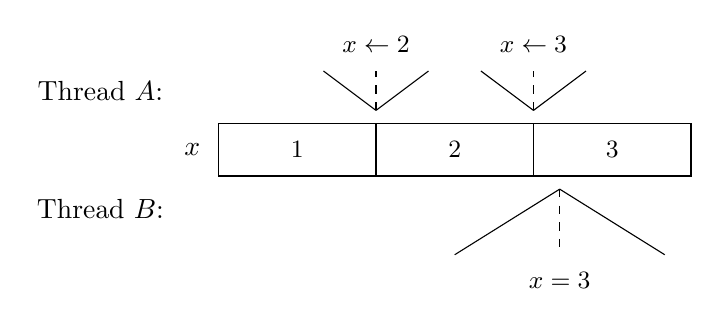
\begin{tikzpicture}
  \node at (-4.5,0.75) { Thread $A$: };
  \node at (-4.5,-0.75) { Thread $B$: };
  \node at (-3.333,0) { $x$ };

  \draw (-3,-0.333) rectangle (-1,0.333) node [midway] { \small $1$ };
  \draw (-1,-0.333) rectangle (1,0.333) node [midway] { \small $2$ };
  \draw (1,-0.333) rectangle (3,0.333) node [midway] { \small $3$ };

  \draw (-1.667,1) -- (-1,0.5) (-1,0.5) -- (-0.333,1);
  \draw [dashed] (-1,0.5) -- (-1,1) node [above=3pt] { \small $x \leftarrow 2$ };

  \draw (0.333,1) -- (1,0.5) (1,0.5) -- (1.667,1);
  \draw [dashed] (1,0.5) -- (1,1) node [above=3pt] { \small $x \leftarrow 3$ };

  \draw (0,-1.333) -- (1.333,-0.5) (1.333,-0.5) -- (2.667,-1.333);
  \draw [dashed] (1.333,-0.5) -- (1.333,-1.333) node [below=3pt] { \small $x = 3$ };
\end{tikzpicture}
}
  \caption{Two threads concurrently (and noninstantaneously) write to and read from a variable.}
\label{figure:time}
\end{figure}

Consider a third example (Figure~\ref{figure:time}) in which two threads $A$ and $B$ interact with a variable $x$ noninstantanously. Invocation is denoted by the leftmost point of an event and completion by the rightmost point. The dotted line indicates the instant at which the operation takes effect. Thread $B$ invokes a read while the value of $x$ is set to $2$. Thread $A$ invokes and completes a write between the time that the read is invoked and the value is actually read. The read operation then returns $3$ even though $x$ was equal to $2$ at the time it was invoked.

While travel time may introduce ambiguity, there are still some restrictions on possible sequences of events. Specifically, an operation cannot take effect before its invocation, nor can it take effect after its completion; rather, it will appear to take effect atomically at some point after it is invoked and before it is completed.

This consistency model is referred to as linearizability (also referred to as atomicity or indivisibility), and it guarantees that the completion of a single operation on a single object will appear to the rest of the system to be instantaneous~\cite{Herlihy1990}. In other words, even though linearizable operations are executed concurrently and take time, they appear to happen in a simple linear order.

\begin{figure}[ht]
  \centering
  \resizebox{0.76\linewidth}{!}{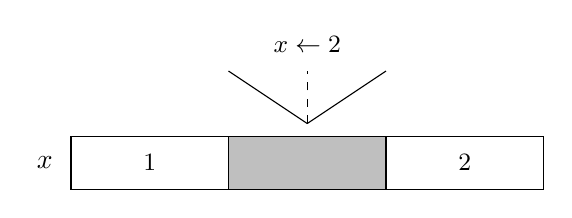
\begin{tikzpicture}
  \node at (-3.333,0) { $x$ };

  \draw (-3,-0.333) rectangle (-1,0.333) node [midway] { \small $1$ };
  \draw [fill=lightgray] (-1,-0.333) rectangle (1,0.333);
  \draw (1,-0.333) rectangle (3,0.333) node [midway] { \small $2$ };

  \draw (-1,1.167) -- (0,0.5) (0,0.5) -- (1,1.167);
  \draw [dashed] (0,0.5) -- (0,1.167) node [above=3pt] { \small $x \leftarrow 2$ };
\end{tikzpicture}
}
  \caption{A single thread performs an atomic write operation on a variable.}
\label{figure:linearizability}
\end{figure}

Figure~\ref{figure:linearizability} demonstrates an atomic write on a variable $x$: Although the operation takes time, the entire operation (denoted by the shaded area) can be collapsed into one apparently instantaneous event. A useful consequence of linearizability is that the results of an operation must be visible as soon as the operation is complete. This can prevent issues such as stale reads (in which a read operation returns a value different from the most recently written value) and non-monotonic reads (in which a later read operation returns an older value than an earlier read operation). Linearizability is also a composable guarantee~\cite{Herlihy1990}---an operation made up of smaller linearizable operations is itself linearizable.

\subsection{Sequential and causal consistency}

For operations to be executed concurrently, they must be able to be executed out of order or in partial order. Lamport, in his foundational work on distributed systems~\cite{Lamport1978}, formalized this by defining a ``happens before'' relation ($\rightarrow$) and its negation ``does not happen before'' ($\nrightarrow$) on a set of operations: If $A$ and $B$ are operations in the same thread and $A$ occurs before $B$, or if $A$ is the sending of a message by one thread and $B$ is the receipt of the same message by another thread, then $A \rightarrow B$. If $A \rightarrow B$ and $B \rightarrow C$, then $A \rightarrow C$. Two operations $A$ and $B$ are said to be concurrent if $A \nrightarrow B$ and $B \nrightarrow A$.

The first condition of the ``happens before'' relation, that $A$ and $B$ are ordered within the same thread, describes sequential consistency. Sequential consistency simply requires that operations in a thread take place in that thread's order. Causal consistency, described by the second condition of the ``happens before'' relation, enforces the intuitive requirement that an effect cannot take place before its cause.

\subsection{Serializable consistency}

A history of operations is said to be serializable if it is equivalent to a serial (i.e., non-interleaved) ordering of its operations~\cite{Herlihy1990}. Serializability is like linearizability in that it demands some linear order of execution. However, serializability describes multiple operations over multiple objects instead of single operations on single objects, and it does not impose any wall-clock time constraints on the history. This means that operations may occur in any order as long as some serial history exists.

\begin{figure}[ht]
  \centering
  \resizebox{0.76\linewidth}{!}{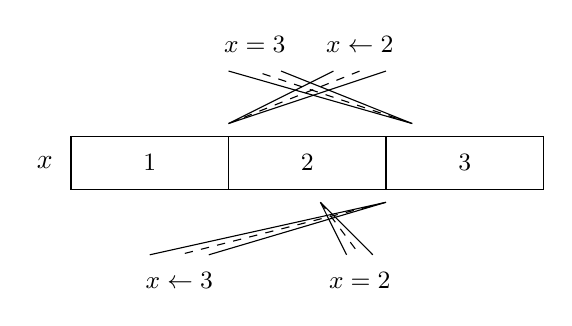
\begin{tikzpicture}
  \node at (-3.333,0) { $x$ };

  \draw (-3,-0.333) rectangle (-1,0.333) node [midway] { \small $1$ };
  \draw (-1,-0.333) rectangle (1,0.333) node [midway] { \small $2$ };
  \draw (1,-0.333) rectangle (3,0.333) node [midway] { \small $3$ };

  \draw (0.333,1.167) -- (-1,0.5) (-1,0.5) -- (1,1.167);
  \draw [dashed] (-1,0.5) -- (0.667,1.167) node [above=3pt] { \small $x \leftarrow 2$ };

  \draw (0.5,-1.167) -- (0.167,-0.5) (0.167,-0.5) -- (0.833,-1.167);
  \draw [dashed] (0.167,-0.5) -- (0.667,-1.167) node [below=3pt] { \small $x = 2$ };

  \draw (-2,-1.167) -- (1,-0.5) (1,-0.5) -- (-1.25,-1.167);
  \draw [dashed] (1,-0.5) -- (-1.625, -1.167) node [below=3pt] { \small $x \leftarrow 3$ };

  \draw (-1,1.167) -- (1.333,0.5) (1.333,0.5) -- (-0.333,1.167);
  \draw [dashed] (1.333,0.5) -- (-0.667,1.167) node [above=3pt] { \small $x = 3$ };
\end{tikzpicture}
}
  \caption{Two threads perform a set of serializable read and write operations on a variable.}
\label{figure:serializability}
\end{figure}

Figure~\ref{figure:serializability} illustrates a set of serializable read and write operations. Even though the executions of each operation occur out of order and even intersect, the events themselves can be arranged serially; no side effects are introduced by the fact that they are executed concurrently.

Serializability alone is a fairly weak consistency model because it does not place any restrictions on time or order~\cite{Kingsbury2014}. Events may happen out of sequence, and, unlike linearizability, serializability is not a composable guarantee. Serializability is useful, though, as a guarantee of isolation: While a serializable set of operations is being executed, it appears to be the only set of operations being executed. For histories to be serializable, then, they must not overlap and cannot interfere with each other.

Linearizability and serializability together guarantee strict serializability, in which a history is equivalent to a serial execution order and that serial order corresponds to the execution order in real time. Given that, linearizability can actually be described as strict serializability restricted to single operations on single objects~\cite{Herlihy1990}.

\section{Common concurrency models}

Modern programming languages generally provide several different concurrency models as tools to reason about concurrent tasks. Swalens et.\ al, in a survey of concurrency models in the Clojure programming language, group commonly used concurrency models into four broad categories: atomic variables, software transactional memory, communicating threads, and proxies~\cite{Swalens2014}.

\subsection{Atomic variables}

Atomic variables are used to share independent objects that do not demand coordinated updates but need to be shared by multiple threads~\cite{Swalens2014}. Atomic variables can only be read and mutated by operations that are guaranteed to be linearizable. For example, the atomic operation \code{compare-and-swap} compares the current value of a variable to a given value and only performs a write if the values are equal~\cite{Swalens2014}. \code{compare-and-swap} ensures that a new value based on outdated information cannot be written: Suppose that a thread $A$ reads a variable $x$ and begins computing a new value. At the same time, another thread $B$ modifies $x$. When $A$ tries to set the value of $x$ via \code{compare-and-swap}, the write will be denied.

Atomic operations are often implemented in hardware and guarantee linearizability at the lowest level possible. \code{fetch-and-add}, another atomic operation, is a common processor instruction that executes multiple hardware-level operations: The old value is copied from a location in memory into a temporary register, addition is performed on the value in the temorary register, and the new value is stored at the original location.

Atomic variables often serve as the basis for higher-level concurrency control mechanisms such as semaphores and locks, which in turn support the implementation of concurrent data structures. A counting semaphore is an atomic variable that serves as a record of how many units of a shared resource, such as a connection or a pooled thread, are available. By taking advantage of atomic operations, the semaphore can be safely updated and will reliably determine whether a shared resource can be used. A single thread can then test if a resource is available and acquire it before proceeding, thereby preventing race conditions~\cite{Swalens2014}. A lock, also referred to as a mutex, guarantees mutual exclusion, which requires that two threads cannot operate on a shared object at the same time. Locks are commonly implemented by a binary semaphore (that is, a semaphore that simply indicates whether a single resource is available).

While lock-based programming is effective, dealing with multiple locks and complex interactions can be cumbersome. One common problem in lock-based programming is resource contention, in which multiple threads vie for control of multiple resources. Suppose, for example, that two threads $A$ and $B$ both require resources $x$ and $y$. $A$ might acquire $x$ and $B$ might acquire $y$. Both would then halt, waiting to acquire a lock on the second needed resource. This type of scenario is commonly referred to as deadlock.

\subsection{Software transactional memory}

Software transactional memory (STM) presents an alternative to lock-based programming by allowing multiple concurrent operations to write to a shared location in memory without securing any kind of lock. STM is an example of optimistic concurrency control: Each thread executes a series of read and write operations (called a transaction) on the shared memory without considering the activity of other threads. On its face, this approach seems disaster-prone---multiple threads writing to the same memory location could easily lead to corrupted data. STM solves this problem by recording all operations in a log. After the entire transaction is completed, the transaction manager verifies that other threads have not also made changes to the shared memory. If there are conflicting changes, the transaction is aborted and retried until it eventually succeeds~\cite{Shavit1995}.

Conceptually, STM simplifies concurrency because it allows a transaction to be thought of as a single strictly serializable operation. A thread cannot observe changes made to other threads while a transaction is in progress, nor can other threads observe modifications by that thread until the transaction has completed successfully. Wrapping a set of operations within a transaction eliminates the need to secure locks, leading to more simple programs. A transaction that modifies several shared variables, for example, would not have to secure locks for all of them. Practically, STM is useful in any situation in which multiple shared objects need to be accessed and modified by multiple threads~\cite{Swalens2014}.

STM also offers significant advantages over lock-based programming in terms of composability. Because a transaction can be viewed as a single linearizable operation, STM can allow any combination of linearizable operations to be composed into a larger linearizable operation. Transactions also enforce modularity by hiding implementation details of the operations within~\cite{Harris2005}.

However, the requirement that transactions must be able to be aborted and retried places constraints on the set of allowed operations. Specifically, a transaction cannot execute any operation that cannot be undone, such as writing to disk or performing a network request. Operations that block indefinitely, like waiting to acquire a lock, may also cause a transaction to fail continuously. STM can also result in a decrease in performance caused by the overhead of maintaining the log and aborting and retrying transactions.

\subsection{Communicating threads}

Other concurrently models avoid the use of shared memory by restricting threads to private memory. Threads communicate strictly by message passing, which avoids issues such as race conditions. Because of the higher level of isolation, communicating threads have long been a solution to describing concurrent operations. Limiting thread communication to message passing also enforces modularity and limits possible negative side effects. A wide variety of communicating thread models exist and are often used to implement event loops or handle communication with external systems~\cite{Swalens2014}.

Communicating sequential processes (CSP), one of the oldest communicating thread models, began as a method of formally describing actions in concurrent systems. CSP describes systems in terms of independent processes that communicate through predefined channels~\cite{Hoare1978}. CSP is notable in that messages are passed synchronously; that is, a sending process will block until a complementary operation is executed on the receiving process~\cite{Swalens2014}. CSP is still widely used in the specification, implementation, and testing of safety-critical systems.

Other models, most notably the actor model, rely on asynchronous message passing to specific entities (actors) rather than named channels~\cite{Agha1986}. Upon receiving a message, an actor can choose to perform an operation on a resource that it controls, send messages to other actors, create new actors, determine the behavior used for the next received message, or ignore the message entirely.

Shared state can also be represented by communicating threads. The agent model, for instance, works similarly to atomic references. A state wrapped by an agent can be modified by a message that sends an updated state. The value can be accessed by a dereferencing operation that reads the current value from the agent~\cite{Swalens2014}.

\subsection{Proxies}

Proxies are a general term used to describe placeholders for values that are the result of some concurrently executed operation. Unlike communicating thread models, which rely on message passing between dedicated threads, a proxy executes some task in a new thread and delivers the result upon completion~\cite{Swalens2014}.

Futures and promises are two of the most common proxy models. The terms are frequently used interchangeably, along with ``delayed,'' ``deferred,'' and ``eventual.'' Generally, futures are resolved to the result of the completed operation. The result is then accessed implicitly; any use of the future will return its value. Promises differ in that they are created as independent objects and require the result to be accessed explicitly.

In practice, proxies are used to execute long-running operations such as rendering or network requests~\cite{Swalens2014} without blocking other operations. For example, to eliminate the need for a program to block on a long network request, a promise could be used to complete the network request in another thread and specify an action that should take place once the result becomes available. Promise objects, which can be easily passed, composed, and chained, offer more flexibility than constructs such as asynchronous callbacks. In fact, many mainstream languages now directly support proxies.

\section{Composability challenges}

Even if a concurrency model guarantees correctness when used alone, issues may arise when it is used with other models. For example, an implementation of an STM that guarantees linearizability assumes that all shared resources are managed by the STM~\cite{Shavit1995}. If such a resource is modified outside of the STM, an unexpected interleaving of operations could result.

Swalens et al.~\cite{Swalens2014} attempted to identify issues that arise when different concurrency models are combined, hoping that future work could identify common ``building blocks'' that could be used to compose a variety of concurrency models. The study surveyed all of the concurrency models available in the Clojure programming language and used them within one another to see what types of correctness issues were encountered.

\subsection{Correctness criteria}

In the study, safety and liveness were used as the two criteria for evaluating the correctness of a combination of models. Together, the two have historically been used to prove the correctness of distributed systems~\cite{Lamport1977}.

Informally, safety guarantees that ``nothing bad will happen.'' In other words, given a correct input, a program will not produce an incorrect result~\cite{Swalens2014}. This property is also referred to as partial correctness. In the context of concurrent programming, safety is generally achieved by the management of shared resources. STM, for instance, only allows shared memory to be accessed through transactions; communicating threads only allow data to be shared through message passing.

Liveness guarantees that ``something good will eventaully happen,'' or that a program will eventually terminate if its input is correct. Taken together, safety and liveness are referred to as total correctness---given a correct input, a program will terminate with the correct output~\cite{Swalens2014}. Deadlocks (in which execution is blocked) and livelocks (in which execution continues indefinitely but never makes progress) are the primary obstacle to liveness and can arise when models are combined.

\subsection{Possible conflicts}

To discover the types of conflicts that might arise when combining different models, the study examined all pairwise combinations of Clojure's models. Using every model within every other model (for example, manipulating an atomic variable within an STM transaction) uncovered the following types of conflicts:

\begin{itemize}
  \item A model might reexecute code containing another concurrency model that performs an irrevocable action. If a block of code such as a transaction were to contain an operation that sent a message on a channel, reexecutions of that block would cause the message to be sent repeatedly.

  \item A model might reexecute code that causes the reexecution to continually happen. The authors of the study observed that, especially when many transactions are being executed at once, a large STM transaction might consistently conflict with another and never succeed.

  \item A model that supports blocking operations might be used within a model that does not expect blocking operations. The authors of the study provided mutually recursive futures as an example---if two futures each attempted to read the value of the other, a deadlock would occur.

  \item A model might not guarantee safety or liveness by design, making safe or live composability impossible.
\end{itemize}

The study noted that some types of bad interactions are prevented by Clojure; as an example, sending a message to an agent from within a transaction is delayed until the transaction succeeds. The study also noted that similar safeguards could prevent other negative interactions. However, preventing every type of negative interaction between models might undermine the purpose of the models to begin with; channels, as mentioned previously, block by design and are inherently incompatible with other models. With that in mind, further research would likely seek to decompose concurrency models into common elements and provide a method to compose those elements safely and efficiently.

\section{Unifying abstractions}

Other research into composable concurrency models has focused on the development of underlying abstractions capable of supporting a wide variety of models. Instead of programmers using composable ``building blocks'' to construct models, these abstractions would make use of those common elements at a lower level to improve performance and interoperability.

\subsection{Ownership-based meta-object protocol}

Marr and D'Hondt~\cite{Marr2012} surveyed a variety of concurrent and parallel programming concepts such as immutability, critical sections, ownership, and common concurrency models to identify a unifying concurrency abstraction that could be implemented in a high-level language virtual machine. A unifying abstraction would enable each concurrency model in a high-level language to be represented in machine code without sacrificing performance or semantics. For instance, a concurrency model in Clojure could be accurately represented by an underlying abstraction in the Java Virtual Machine, and code written in the Java programming language could interact with that model correctly. To identify the concepts that would need to be supported at the virtual machine level, Marr and D'Hondt selected four questions:

\begin{enumerate}
  \item Can the concept be reasonably implemented as a library? A library implementation may suffer from loss of performance or semantics to an extent that the concept would warrant virtual machine inclusion.

  \item Does the concept require runtime support to guarantee its semantics? Semantic guarantees may be enforced by a compiler but not the virtual machine. For example, immutable objects in one language may not be immutable in machine code, and therefore may be mutated by another language.

  \item Would runtime support benefit performance? Deeper knowledge of the concept may enable the virtual machine to better optimize. Some concepts, though, may require knowledge of the underlying hardware to realize any performance improvements; such concepts would not necessarily benefit from runtime support.

  \item Is the concept already supported by a common virtual machine like the Java Virtual Machine or the Common Language Runtime?
\end{enumerate}

From those questions, 26 concepts were identified that would benefit from runtime support. Of those, 18 suffered from loss of semantic guarantees when compiled to machine code; the survey mentioned transactions as an example. With those concepts in mind, Marr and D'Hondt derived the following requirements for a unifying abstraction:

\begin{itemize}
  \item Managed mutation and execution: A model may impose rules on how objects can be modified; therefore, mutation must be handled in a way that allows those rules to be enforced. By way of example, a thread should not be permitted to mutate a variable that a model declares immutable. Similarly, a model may restrict the invocation of operations on objects.

  \item Ownership: All mutation and execution on an object is regulated relative to some ``owning'' entity, so ownership should be supported in a way that allows for adaptable mutation and execution rules.

  \item Leveled reflection: Reflection allows a program to examine its own structure and behavior at runtime. To guarantee safety, there needs to be a distinction between language-level reflection (reflection operations supported by the high-level language) and meta-level reflection (reflection operations on the low-level abstraction).

  \item Enforceability: All defined restrictions should be enforceable on different concurrency models. Additionally, the semantics of the language (immutability, for example) in which a model is defined must be enforced regardless of where the model is used.
\end{itemize}

\begin{figure}[ht]
  \centering
  \resizebox{0.55\linewidth}{!}{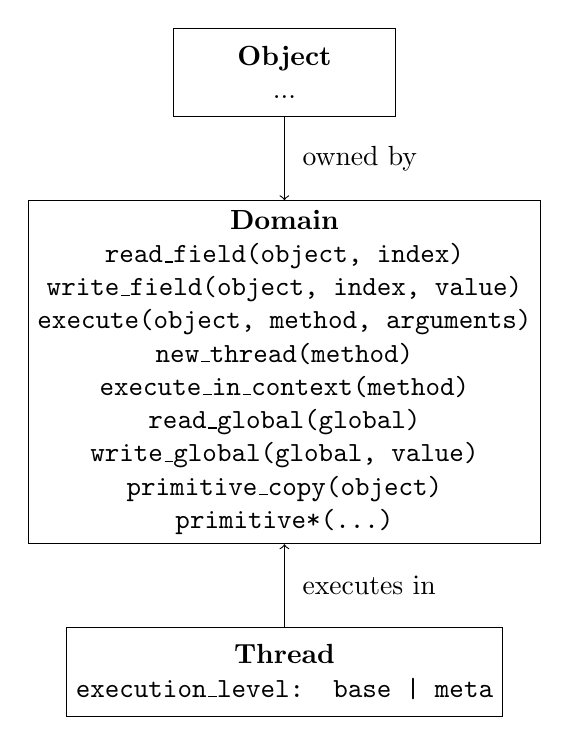
\begin{tikzpicture}
  \node at (0,0) [align=center,draw] (domain) {
    \textbf{Domain}\\
    \code{read\_field(object, index)}\\
    \code{write\_field(object, index, value)}\\
    \code{execute(object, method, arguments)}\\
    \code{new\_thread(method)}\\
    \code{execute\_in\_context(method)}\\
    \code{read\_global(global)}\\
    \code{write\_global(global, value)}\\
    \code{primitive\_copy(object)}\\
    \code{primitive*(...)}
  };

  \node [align=center,draw,above=30pt of domain,minimum height=3.2em,minimum width=80pt] (object) {
    \textbf{Object}\\
    ...
  };

  \node [align=center,draw,below=30pt of domain,minimum height=3.2em,minimum width=80pt] (thread) {
    \textbf{Thread}\\
    \code{execution\_level: base | meta}
  };

  \draw[->] (object.south) -- node[right=3pt] {owned by} (domain.north);
  \draw[->] (thread.north) -- node[right=3pt] {executes in} (domain.south);
\end{tikzpicture}
}
  \caption{Marr and D'Hondt's owenership-based meta-object protocol~\cite{Marr2012}.}
\label{figure:obmop}
\end{figure}

Given those requirements, Marr and D'Hondt defined an ownership-based meta-object protocol (MOP) that could describe a low-level abstraction, illustrated in Figure~\ref{figure:obmop}. The owner of an object, referred to as the domain, manages operations on all of the objects that it owns. Specifically, the domain handles all reading and writing of object fields and invocation of methods on objects. This satisfies the ownership requirement. Read and write operations are directed to the \code{read\_field} and \code{write\_field} operations on the domain, satisfying the managed mutation requirement. Similarly, all method invocations are directed to the \code{exec}, satisfying the managed execution requirement. Threads are executed in a domain and specify whether execution occurs at the language level with restricted reflection or the meta level with unrestricted reflection, satisfying the leveled reflection requirement. Globally shared resources are handled by the domain (through the \code{read\_global} and \code{write\_global} methods) if they might break semantics. Additionally, the \code{primitive*} operations allow callers to override the semantics of virtual machine primitives, completing the enforcability requirement.

To demonstrate the suitability of the MOP as a low-level abstraction, Marr and D'Hondt implemented several concurrency models. The MOP was able to support LRSTM (a STM for the Smalltalk language), Clojure's agents (which rely on communicating threads), active objects (a variation on proxies), and several other models. While the MOP was able to successfully enforce the semantics of each model, the resulting performance cost suggested that the MOP must be implemented at the virtual machine level to sufficiently reduce the overhead of abstraction. Marr and D'Hondt also note that regarding the owner of an object as the only entity able to restrict interaction is somewhat limiting. For instance, the behavior of the system when different semantics interact needs to be explicitly specified.

\section{Conclusion}

There are a rich variety of concurrency models that can be used to represent concurrent tasks, abstract over low-level details, and ensure that concurrent applications perform correctly. Recent research has attempted to identify ways in which these models can be safely used together, common features of these models, and underlying abstractions capable of representing many different models.

Future work will likely explore ways in which concurrency models can be decomposed and recomposed from common elements. This, in turn, would lead to the development of more generalized ways of describing concurrency models and perhaps additional unifying abstractions. As Marr and D'Hondt note, a ``silver bullet'' does not exist. However, there is certainly promise in searching for better ways to represent concurrent operations.

\section*{Acknowledgments}

Thanks to Elena Machkasova, K.~K. Lamberty, and Matthew Justin for their suggestions and feedback.

\printbibliography{}

\end{document}
